\documentclass[12pt,a4paper]{report}

\usepackage[utf8]{inputenc}
\usepackage[T1]{fontenc}
\usepackage[margin=3cm]{geometry}
\usepackage{amsmath,amssymb}
\usepackage{graphicx}
\usepackage{hyperref}
\usepackage{booktabs}
\usepackage{setspace}
\usepackage{tikz}
\usepackage{caption}
\usepackage{subcaption}
\usepackage{algorithm}
\usepackage{algpseudocode}
\usepackage[style=ieee]{biblatex}

\onehalfspacing

\title{A Computational Framework for Multi-Agent Reinforcement Learning
       in Partially Observable Environments}
\author{John Smith}
\date{}

\begin{document}

\maketitle

\begin{abstract}
Multi-agent reinforcement learning (MARL) in partially observable environments presents unique
challenges due to the combinatorial explosion of joint state-action spaces and the non-stationarity
introduced by concurrently learning agents. This thesis proposes a novel framework, MARL-PO,
that addresses these challenges through a combination of decentralized execution with centralized
training, attention-based communication protocols, and curriculum learning strategies.
\end{abstract}

\tableofcontents

\chapter{Introduction}
\label{ch:intro}

Reinforcement learning (RL) has achieved remarkable success in single-agent domains such as game
playing and robotic control. However, many real-world problems involve multiple agents that must
coordinate their actions in environments where each agent has only a partial view of the global state.

\section{Motivation}
Consider a fleet of autonomous vehicles navigating an urban environment. Each vehicle has access
only to its local sensor readings---nearby vehicles, pedestrians, traffic signals---while the global
state encompasses the entire traffic network. The challenge is to learn policies that are both
locally executable and globally coherent.

\section{Problem Formulation}
We formalize the problem as a Decentralized Partially Observable Markov Decision Process (Dec-POMDP)
\cite{oliehoek2016concise}, defined by the tuple:

\begin{equation}
\mathcal{M} = \langle \mathcal{S}, \{\mathcal{A}_i\}_{i=1}^n, \{\mathcal{O}_i\}_{i=1}^n,
    \mathcal{T}, \mathcal{R}, \gamma \rangle
\label{eq:dec_pomdp}
\end{equation}

where $\mathcal{S}$ is the global state space, $\mathcal{A}_i$ is the action space of agent $i$,
$\mathcal{O}_i$ is the observation space of agent $i$, $\mathcal{T}: \mathcal{S} \times \mathcal{A}_1 \times \cdots \times \mathcal{A}_n \rightarrow \Delta(\mathcal{S})$ is the transition function,
$\mathcal{R}: \mathcal{S} \times \mathcal{A}_1 \times \cdots \times \mathcal{A}_n \rightarrow \mathbb{R}$
is the shared reward function, and $\gamma \in [0, 1)$ is the discount factor.

\section{Contributions}
The primary contributions of this thesis are:
\begin{enumerate}
    \item A formal characterization of the credit assignment problem in MARL under partial observability.
    \item The MARL-PO framework, which combines three key mechanisms:
    \begin{itemize}
        \item Centralized training with decentralized execution (CTDE)
        \item Multi-head attention for inter-agent communication
        \item Automated curriculum learning for progressive task difficulty
    \end{itemize}
    \item Extensive empirical evaluation on cooperative navigation, predator-prey, and StarCraft micromanagement benchmarks.
\end{enumerate}

\chapter{Background}
\label{ch:background}

\section{Reinforcement Learning}
In single-agent RL, an agent interacts with an environment modeled as a Markov Decision Process (MDP).
At each timestep $t$, the agent observes state $s_t$, selects action $a_t \sim \pi(\cdot \mid s_t)$,
receives reward $r_t$, and transitions to $s_{t+1}$. The objective is to maximize the expected
discounted return:

\begin{equation}
J(\pi) = \mathbb{E}_{\tau \sim \pi}\left[\sum_{t=0}^{\infty} \gamma^t r_t\right]
\label{eq:rl_objective}
\end{equation}

\section{Policy Gradient Methods}
Policy gradient methods directly optimize the policy parameters $\theta$ by ascending the gradient
of the expected return:

\begin{equation}
\nabla_\theta J(\theta) = \mathbb{E}_{\tau \sim \pi_\theta}\left[
    \sum_{t=0}^{T} \nabla_\theta \log \pi_\theta(a_t \mid s_t) \hat{A}_t
\right]
\label{eq:policy_gradient}
\end{equation}

where $\hat{A}_t$ is an estimate of the advantage function. Proximal Policy Optimization (PPO)
\cite{schulman2017proximal} stabilizes training by clipping the policy update:

\begin{equation}
\mathcal{L}^{\text{CLIP}}(\theta) = \mathbb{E}_t\left[
    \min\left(
        r_t(\theta) \hat{A}_t,\;
        \text{clip}(r_t(\theta), 1 - \epsilon, 1 + \epsilon) \hat{A}_t
    \right)
\right]
\label{eq:ppo_clip}
\end{equation}

\chapter{The MARL-PO Framework}
\label{ch:framework}

\section{Architecture Overview}
The MARL-PO framework consists of three interconnected components:

\begin{figure}[htbp]
    \centering
    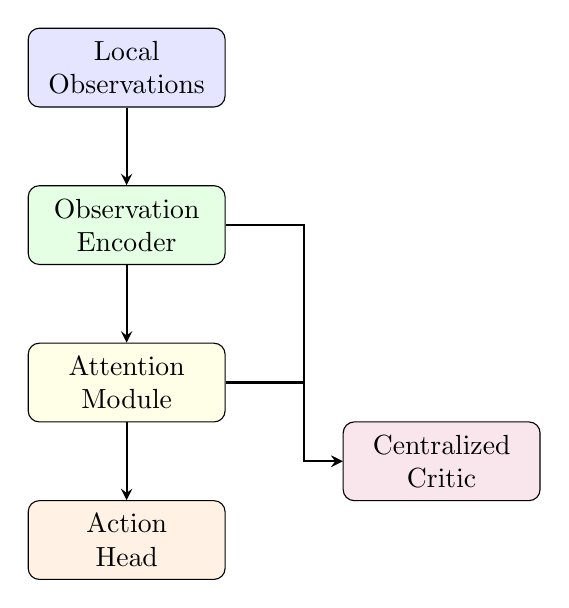
\begin{tikzpicture}[
        box/.style={draw, rounded corners, minimum width=2.5cm, minimum height=1cm, align=center},
        arrow/.style={->, >=stealth, thick}
    ]
        \node[box, fill=blue!10] (obs) at (0, 4) {Local\\Observations};
        \node[box, fill=green!10] (enc) at (0, 2) {Observation\\Encoder};
        \node[box, fill=yellow!10] (att) at (0, 0) {Attention\\Module};
        \node[box, fill=orange!10] (act) at (0, -2) {Action\\Head};
        \node[box, fill=purple!10] (crit) at (4, -1) {Centralized\\Critic};

        \draw[arrow] (obs) -- (enc);
        \draw[arrow] (enc) -- (att);
        \draw[arrow] (att) -- (act);
        \draw[arrow] (enc.east) -- ++(1, 0) |- (crit);
        \draw[arrow] (att.east) -- ++(1, 0) |- (crit);
    \end{tikzpicture}
    \caption{MARL-PO agent architecture}
    \label{fig:architecture}
\end{figure}

\section{Attention-Based Communication}
Agents communicate through a multi-head attention mechanism. Given agent $i$'s encoded observation
$\mathbf{h}_i$, the attention-weighted message from agent $j$ is:

\begin{align}
\mathbf{q}_i &= \mathbf{W}_q \mathbf{h}_i \\
\mathbf{k}_j &= \mathbf{W}_k \mathbf{h}_j \\
\mathbf{v}_j &= \mathbf{W}_v \mathbf{h}_j \\
\alpha_{ij} &= \frac{\exp(\mathbf{q}_i^\top \mathbf{k}_j / \sqrt{d_k})}
                    {\sum_{l} \exp(\mathbf{q}_i^\top \mathbf{k}_l / \sqrt{d_k})} \\
\mathbf{m}_i &= \sum_j \alpha_{ij} \mathbf{v}_j
\label{eq:attention}
\end{align}

\section{Curriculum Learning}
We employ an automated curriculum that progressively increases environment difficulty based on agent
performance. The difficulty parameter $d \in [0, 1]$ controls:
\begin{itemize}
    \item Number of agents in the environment
    \item Size of the navigation area
    \item Density of obstacles
    \item Observation noise magnitude
\end{itemize}

The curriculum advances when the mean episode return exceeds a threshold $\tau$ for $K$ consecutive
evaluations:

\begin{equation}
d_{t+1} = \begin{cases}
    \min(d_t + \delta, 1) & \text{if } \bar{R}_{t-K:t} > \tau \\
    d_t & \text{otherwise}
\end{cases}
\label{eq:curriculum}
\end{equation}

\chapter{Experiments}
\label{ch:experiments}

We evaluate MARL-PO against state-of-the-art MARL algorithms: MADDPG, QMIX, MAPPO, and COMMNET.

\begin{table}[htbp]
    \centering
    \caption{Mean episode return on cooperative navigation (5 runs, $\pm$ std)}
    \label{tab:navigation}
    \begin{tabular}{@{}lccc@{}}
        \toprule
        Algorithm & 3 Agents & 5 Agents & 10 Agents \\
        \midrule
        MADDPG    &  $-45.2 \pm 8.1$ & $-78.4 \pm 12.3$ & $-156.7 \pm 21.4$ \\
        QMIX      &  $-38.9 \pm 6.7$ & $-65.2 \pm 9.8$  & $-128.3 \pm 18.2$ \\
        MAPPO     &  $-32.1 \pm 5.2$ & $-54.7 \pm 8.4$  & $-102.5 \pm 15.6$ \\
        MARL-PO   &  $\mathbf{-24.7 \pm 3.8}$ & $\mathbf{-41.3 \pm 6.1}$ & $\mathbf{-78.9 \pm 10.4}$ \\
        \bottomrule
    \end{tabular}
\end{table}

\chapter{Conclusion}
\label{ch:conclusion}

This thesis presented MARL-PO, a framework for multi-agent reinforcement learning in partially
observable environments. By combining CTDE with attention-based communication and curriculum
learning, MARL-PO achieves state-of-the-art performance across diverse benchmarks.

\bibliographystyle{plain}
\begin{thebibliography}{9}

\bibitem{oliehoek2016concise}
F.~Oliehoek and C.~Amato.
\newblock \emph{A Concise Introduction to Decentralized POMDPs}.
\newblock Springer, 2016.

\bibitem{schulman2017proximal}
J.~Schulman, F.~Wolski, P.~Dhariwal, A.~Radford, and O.~Klimov.
\newblock Proximal policy optimization algorithms.
\newblock \emph{arXiv preprint arXiv:1707.06347}, 2017.

\end{thebibliography}

\end{document}
